% !TeX encoding = UTF-8
% !TeX program = pdflatex
% !BIB program = bibtex
%
% DRAFT — Autonomous Systems A / CPS Laboratory Final Report, Group 4
% Template/setup follows Machine_Learning_for_CPS_Riwaj_Ghimire (local lni.cls + lni.bst, bibtex).
% Sections marked with %% TODO need team input before submission.
\documentclass[english]{lni}

\usepackage{graphicx}
\usepackage{float}
\usepackage{booktabs}
\usepackage{listings}
\usepackage{needspace}
\usepackage{array}
\newcolumntype{L}[1]{>{\raggedright\arraybackslash\hyphenpenalty=10000\exhyphenpenalty=10000}p{#1}}
\usepackage{draftwatermark}
\SetWatermarkText{Autonomous Systems A - SummerTerm 2026}
\SetWatermarkLightness{0.98}
\SetWatermarkScale{0.25}

\begin{document}

\title[Autonomous Systems A Lab Final Report]{Machine Learning Modelled Autonomous Driving and CPS In Truck Platooning.}
\author[Bertrand Mungu Cho, Daniel Chidi Chimezie, Riwaj Ghimire, Stephen Uzochi Obuh]{Bertrand Mungu Cho, Daniel Chidi Chimezie, Riwaj Ghimire, Stephen Uzochi Obuh\footnote{Hamm-Lippstadt University of Applied Sciences, \email{bertrand-mungu.cho@stud.hshl.de, daniel-chidi.chimezie@stud.hshl.de, riwaj.ghimire@stud.hshl.de, stephen-uzochi.obuh@stud.hshl.de}}}
\startpage{1}
\booktitle{Autonomous Systems A Lab Final Report}
\year{Summer Term 2026}

\maketitle
\setcounter{tocdepth}{1}
\tableofcontents

\newpage

\begin{abstract}
This report documents the work completed by Group~4 in the Autonomous Systems~A module, which consisted of two connected laboratories: a machine learning lab and a cyber-physical systems lab, both motivated by truck platooning and advanced driver assistance systems. In the machine learning lab, a line-following system for a single vehicle was developed: camera frames are reduced to a compact six-dimensional feature representation using OpenCV, and a support vector regressor predicts a continuous steering command that is smoothed by a PD controller. Trained on 17{,}046 frames recorded in the Science Truck, the tuned model reaches a test mean absolute error of 0.0075 ($R^2 = 0.99$) under a strictly temporal evaluation protocol and placed among the top teams in the final line-following competition. The cyber-physical systems lab builds on this single-vehicle capability and addresses the coordination of an entire platoon: four operational scenarios (platoon formation, emergency braking, communication failure, and platoon splitting) were described with functional, timing, and safety requirements, modelled in SysML/UML, and translated into timed automata. An integrated UPPAAL model combining lead-truck control, follower control, distance keeping, and communication monitoring was simulated and formally verified; the model is proven deadlock-free.
\end{abstract}

\newpage

\section{Motivation}
In truck platooning, several trucks are electronically coupled into a closely spaced convoy that is coordinated over vehicle-to-vehicle (V2V) communication. This promises lower fuel consumption through reduced aerodynamic drag, better road utilisation, and improved safety, because machine reaction times replace human ones \cite{LBS22}. At the same time, platooning is a safety-critical cyber-physical system: a lost brake message or an insufficient following gap can directly cause a multi-vehicle collision. Careful requirements engineering and formal verification are therefore essential.

The module approached this problem domain in two connected laboratories. The machine learning lab addressed the perception and control of a single vehicle: before trucks can drive in a platoon at all, each vehicle must be able to follow its lane reliably. This was implemented as a machine-learning-based line follower and validated on the Science Truck platform in a competitive setting (Section~\ref{sec:svm}). The cyber-physical systems lab then moved from the single vehicle to the coordination of an entire platoon: the relevant scenarios and requirements were specified (Section~\ref{sec:scenarios}), the required communication between the trucks was defined (Section~\ref{sec:comm}), and the resulting control behaviour was modelled as a network of timed automata and verified with UPPAAL (Section~\ref{sec:uppaal}). This report documents both labs together, since they form one continuous development path from a single autonomous vehicle to a verified platooning concept.

\section{Project Organisation}\label{sec:org}
The work was organised with version control on a shared GitHub repository. The machine learning lab ran first, with fixed weekly deadlines in May: lab exercises, data collection in the Science Truck, model refinement, and the final competition on May~22. The cyber-physical systems lab followed in milestone-based development steps: Milestone~1 (June~4) covered scenario identification and SysML modelling, Milestone~2 (June~11) the communication data and protocols, Milestone~3 (June~18) the control behaviour, and Milestone~5 (June~25) the integrated simulation. Every member contributed to both labs. In the machine learning lab, the line-following pipeline was divided into four stages, each owned by one member; in the cyber-physical systems lab, each member owned one platooning scenario end to end. The final presentation and this report were joint work. Table~\ref{tab:team} summarises the roles and responsibilities.

\begin{table}[H]
\centering
\caption{Team members and responsibilities in both labs.}
\label{tab:team}
\renewcommand{\arraystretch}{1.6}
\setlength{\tabcolsep}{5pt}
\begin{tabular}{L{3.3cm}L{2.0cm}L{2.9cm}L{3.0cm}}
\toprule
Member & Role & ML lab stage & CPS lab scenario \\
\midrule
Daniel Chidi Chimezie (1230515) & Project Manager & Science Truck data collection, dataset preparation & Communication failure; coordination of shared channels \\
Riwaj Ghimire   (1232171) & DevOps Manager & Feature pipeline and SVR training & Emergency braking and UPPAAL model \\
Stephen Uzochi Obuh (2210044) & System Integration Lead & Hyperparameter tuning and ROS\,2 deployment & Platoon splitting; integration of the combined model \\
Bertrand Mungu Cho (2220052) & Verification and Testing Lead & Model testing and evaluation & Platoon formation; deadlock-freedom verification \\
\bottomrule
\end{tabular}
\renewcommand{\arraystretch}{1}
\end{table}

\section{SVR-Based Line Following}\label{sec:svm}

\subsection{Approach and Feature Extraction}
The task is to steer a vehicle along a green line painted on the road using only a front camera ($1280 \times 720$, approx.\ 30\,fps). Instead of feeding raw pixels to a learning algorithm, the image is reduced with OpenCV to a compact geometric description of the line: (1)~a perspective-correct trapezoidal region of interest, measured from real frames, restricts processing to the road surface; (2)~an HSV colour threshold with morphological opening and closing isolates the green line; (3)~the horizontal line position is sampled at three heights of the trapezoid (bottom, middle, top) using adaptive row scanning. Each frame is thereby described by six features: three offsets of the line relative to the calibrated vehicle centre, normalised to $[-1, 1]$, and three validity flags that indicate whether the corresponding band actually contained the line. The flags prevent the model from misinterpreting a missing detection as ``line centred''. Figure~\ref{fig:mask-pipeline} shows the pipeline stages on an actual frame; Figure~\ref{fig:app-label} in the appendix shows the resulting label overlaid on a driving frame.

\begin{figure}[H]
\centering
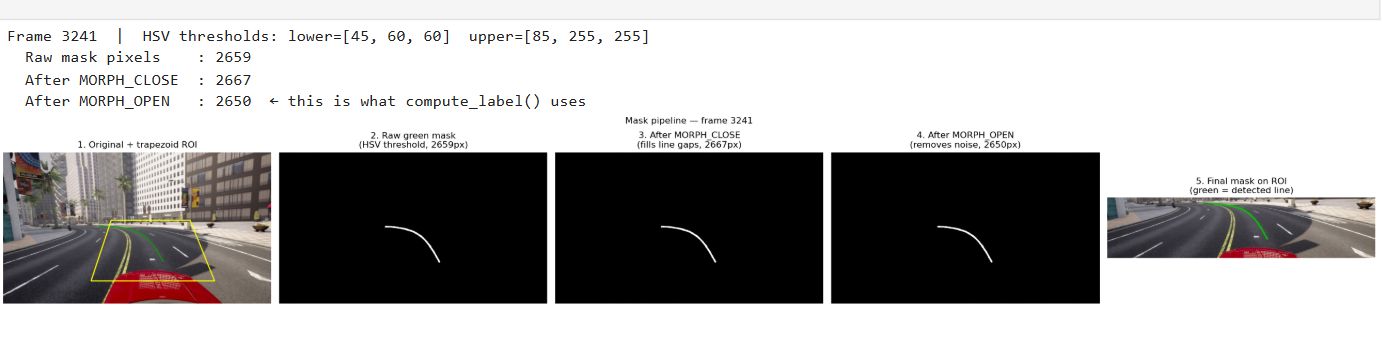
\includegraphics[width=0.95\textwidth]{figures/appendix_mask_pipeline.png}
\caption{Feature extraction pipeline on a single frame: trapezoid ROI, raw HSV green mask, mask after morphological closing and opening, and the final detected line.}
\label{fig:mask-pipeline}
\end{figure}

\needspace{4\baselineskip}
Training labels are continuous steering targets in $[-1, 1]$ computed by a geometric formula that blends the three offsets, with case-dependent weights for straight driving, approaching curves, and cross-over situations. Formulating the problem as regression rather than classification yields smooth steering instead of coarse left/straight/right decisions.

\subsection{Training and Evaluation}
The dataset consists of 17{,}046 consecutive frames recorded in the Science Truck (label distribution in Figure~\ref{fig:app-dist}). Because neighbouring video frames are nearly identical, a random train/test split would leak information; the last 20\,\% of frames (3{,}410) were therefore held out as a contiguous temporal block, and hyperparameter search used \texttt{TimeSeriesSplit} cross-validation so that validation frames always lie after training frames. Support vector machines remain a well-validated choice for real-time, sensor-driven driving-safety classification tasks, for example in recent work on road surface condition classification \cite{MP24}; an RBF support vector regressor within a \texttt{StandardScaler} pipeline was tuned by grid search (36 candidates, 5 temporal folds). Curve frames ($|$label$| > 0.15$) received a threefold sample weight to counteract the dominance of straight-driving frames.

\begin{table}[H]
\centering
\caption{Evaluation results.}
\label{tab:svm-results}
\renewcommand{\arraystretch}{1.6}
\setlength{\tabcolsep}{5pt}
\begin{tabular}{L{4.6cm}L{1.7cm}L{1.5cm}L{2.9cm}}
\toprule
Model & MAE & $R^2$ & Evaluated on \\
\midrule
Baseline SVR (default parameters) & 0.0198 & 0.9502 & 3{,}410 held-out frames \\
Tuned SVR ($C{=}5$, $\gamma{=}0.1$, $\varepsilon{=}0.01$) & \textbf{0.0075} & \textbf{0.9909} & 17{,}046 frames (full dataset) \\
\bottomrule
\end{tabular}
\renewcommand{\arraystretch}{1}
\end{table}

The baseline was evaluated on the 3{,}410-frame held-out test block as a quick sanity check before tuning. After grid search, the tuned model was retrained on the full dataset and exported as a single pickle pipeline; tuning reduced the mean absolute error by 62\,\% (Table~\ref{tab:svm-results} and Figure~\ref{fig:tuned-model}); the baseline predicted-versus-true plot is shown in Figure~\ref{fig:app-baseline} in the appendix. A permutation importance test confirmed that all three offset features carry substantial signal (MAE increase of $+0.025$ to $+0.045$ when shuffled, Figure~\ref{fig:app-importance}), while the validity flags act as auxiliary context.

\begin{figure}[H]
\centering
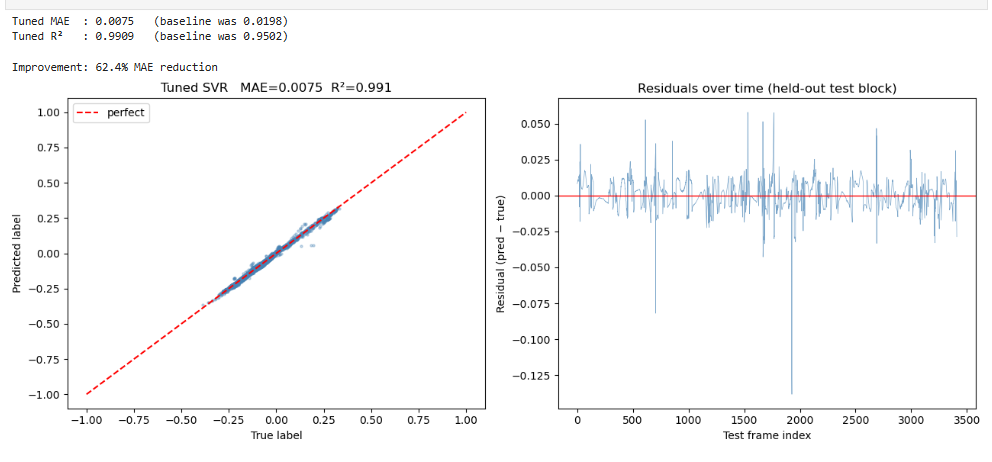
\includegraphics[width=0.95\textwidth]{figures/appendix_tuned_model.png}
\caption{Predicted versus true steering label for the tuned SVR (left) and residuals over the held-out test block (right).}
\label{fig:tuned-model}
\end{figure}

\subsection{Deployment and Competition}
At runtime, the deployed ROS\,2 node extracts the six features from each frame, predicts a steering offset with the SVR, and passes it through a PD controller whose gains are selected from a throttle-dependent table: higher speeds use a lower proportional gain and a higher derivative gain to avoid overshoot and oscillation. Robustness measures include rejection of compact noise blobs via a row-span test, holding the last steering command for up to ten frames when the line is briefly lost, and a neutral-steering fallback with an alert if the line remains undetected. In the final line-following competition in the Science Truck (May~22), the system placed among the top teams.
%% TODO: insert exact placement / lap results if desired.

\subsection{Challenges and Solutions}
Several design choices in Sections~2.1--2.3 are the direct result of problems found while working with real camera data, not decisions made in advance.

\textbf{Noise from the environment.} An early version of the detector used a simple colour mask over the full image. In practice this also picked up green-tinted reflections and foliage in the background, which produced short, compact blobs of colour that were mistaken for the line. The fix was twofold: restricting detection to a perspective-correct trapezoidal region of interest so only the road surface in front of the vehicle is considered, and adding a row-span check that rejects any detected blob not tall enough to plausibly be the line, even on a sharp turn.

\textbf{Data leakage in evaluation.} The first evaluation attempt used a random train/test split, which produced deceptively good scores because neighbouring video frames are nearly identical and a frame in the training set could be adjacent to an almost-copy of itself in the test set. This was identified as invalid before the numbers were used for tuning, and the evaluation protocol was changed to a temporal block split combined with \texttt{TimeSeriesSplit} cross-validation, so that every validation frame comes strictly after the frames used to train it, matching how the model is actually used at inference time.

\textbf{Underfitting on sharp turns.} The initial tuned model achieved a low overall MAE but still steered too weakly through sharp curves, because straight-driving frames vastly outnumber curve frames in the dataset and dominate the loss function. Testing on the vehicle made this failure mode visible even though the aggregate metric looked acceptable. The solution was to reweight the training loss, giving curve frames ($|$label$| > 0.15$) three times the weight of straight frames, which brought the test MAE down from 0.0198 to 0.0075 while specifically correcting the sharp-turn behaviour rather than the average case.

\textbf{Missing detections.} Because the line is sampled at three separate heights, any one band can legitimately be empty, for example a corner where only the bottom part of the line is visible. Feeding a plain zero for a missing band would be indistinguishable from a genuinely centred line at that height. This was solved by adding three binary validity flags to the feature vector, so the regressor can tell a real reading of zero apart from a missing one.

\section{Truck Platooning: Scenarios and Requirements}\label{sec:scenarios}
The machine learning lab ends with a single truck that can follow its lane reliably. The cyber-physical systems lab starts from exactly this point and asks what changes when several such trucks drive together as a platoon. Lane keeping alone is then no longer sufficient: the trucks must exchange information over V2V communication, react to each other within guaranteed times, and remain safe when this communication fails. Unlike the line follower, these properties cannot be validated by test drives alone, because the critical situations (an emergency stop at full speed, a communication blackout) are exactly the ones that must not be provoked on a real road. The platooning behaviour was therefore specified through scenarios and requirements and verified formally with model checking in the following sections.

Four operational scenarios were identified, one per team member. Each scenario was documented with preconditions, trigger events, main, alternative and exception flows, and functional, timing, and safety requirements, and modelled with SysML/UML diagrams.

\needspace{8\baselineskip}
\subsection{Platoon Formation}
A lead truck broadcasts a platoon advertisement (speed, position, lane, formation intent). Candidate followers submit join requests with their identity, capabilities, and position; a platoon manager validates them against safety policies before assigning platoon position, role, and target gap (Figure~\ref{fig:formation-seq}). A coordinated manoeuvre then brings the vehicles into formation. Key timing requirements: advertisement reception $\leq 200$\,ms, join-request forwarding $\leq 100$\,ms, join decision $\leq 500$\,ms, formation completion $\leq 1$\,s. The corresponding SysML requirement diagram is included in the appendix (Figure~\ref{fig:app-formation-req}).

\begin{figure}[H]
\centering
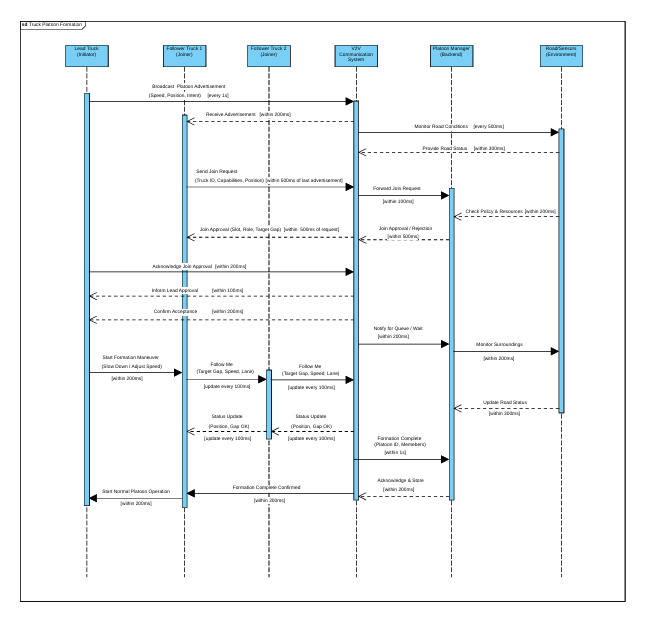
\includegraphics[width=0.6\textwidth]{figures/platoon_formation_sequence.png}
\caption{Sequence diagram of the platoon formation scenario.}
\label{fig:formation-seq}
\end{figure}

\subsection{Emergency Braking}
When the lead truck detects an obstacle within critical stopping distance, it applies maximum braking and simultaneously broadcasts an emergency brake signal over V2V, so that all followers brake without human reaction delay (Figure~\ref{fig:eb-diagrams}). This design follows recent findings that V2V-based emergency braking allows substantially shorter safe inter-vehicle distances and faster response than a radar-only automatic emergency braking system, even under conservative assumptions on communication reliability \cite{STS22}. If V2V is unavailable, followers fall back to onboard sensor-based collision avoidance, which is a degraded but still safe mode with larger stopping distances. The safety requirements SR-EB-01 to SR-EB-06 bound the timing chain: hazard detection to brake activation $\leq 50$\,ms, broadcast latency $\leq 100$\,ms, follower brake activation $\leq 150$\,ms after signal reception, sensor-based fallback within $200$\,ms, and full platoon stop within $5$\,s; deceleration must remain below the jackknifing limit, and a braking failure of one truck must not cascade into a chain collision.

\begin{figure}[H]
\centering
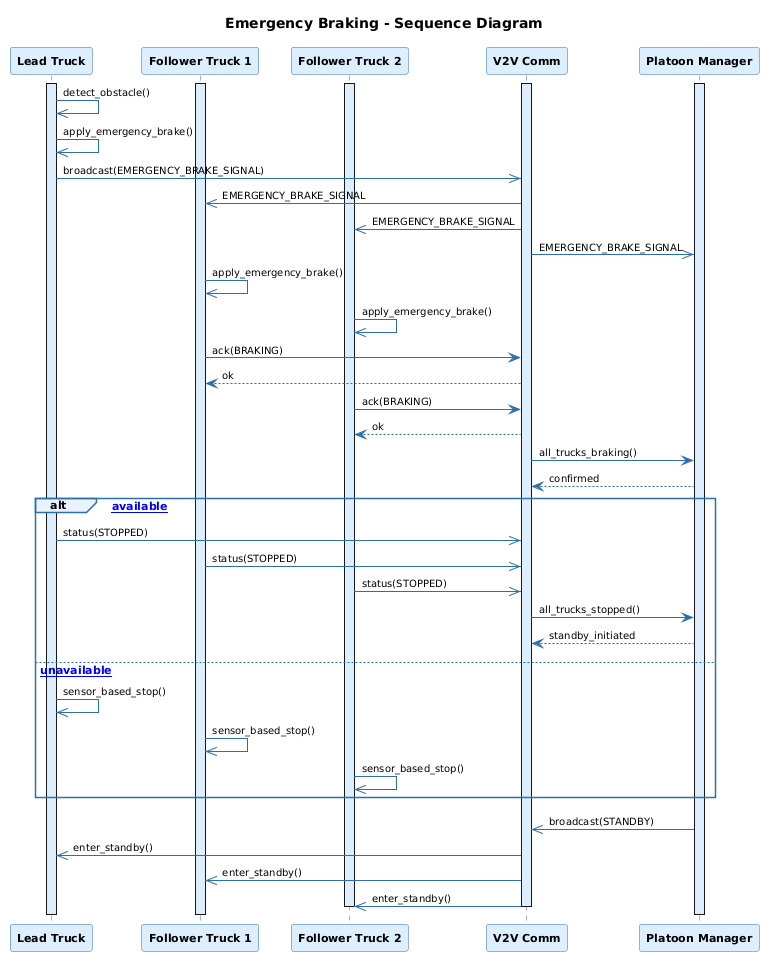
\includegraphics[width=0.6\textwidth]{figures/emergency_braking_sequence.png}
\caption{Sequence diagram of the emergency braking scenario.}
\label{fig:eb-diagrams}
\end{figure}

\subsection{Communication Failure}
V2V communication may fail due to network outages, hardware faults, interference, or software errors. A communication watchdog monitors heartbeat and status messages; when the timeout threshold is exceeded, the failure is confirmed and the affected trucks enter a fail-safe mode in which safe following distances are enforced and road safety is prioritised over platoon efficiency (Figure~\ref{fig:comm-failure}). Reconnection is attempted periodically, and normal operation resumes once communication is restored. Safety requirements demand failure detection within the configured timeout, guaranteed fail-safe entry, alarm generation, and availability of emergency braking in every communication state.

\begin{figure}[H]
\centering
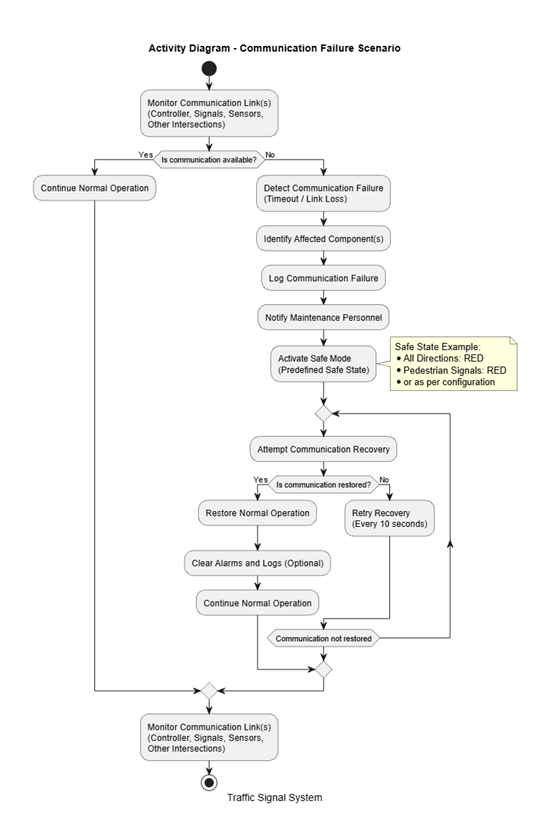
\includegraphics[width=0.62\textwidth]{figures/communication_failure_activity.png}
\caption{Activity diagram of the communication failure scenario.}
\label{fig:comm-failure}
\end{figure}

\subsection{Platoon Splitting}
Together with merging, splitting is one of the fundamental operations of platooning, defined in the literature as separating a long platoon into scattered vehicles or shorter sub-platoons, with operation safety as the primary design objective \cite{LCL22}. Approaching a route divergence, a platoon of one leader and three followers must split into two independent sub-platoons (Figures~\ref{fig:splitting-req} and~\ref{fig:splitting-usecase}). The manoeuvre proceeds in six phases: route divergence detection, split negotiation (including promotion of a follower to leader of the second sub-platoon), gap creation (2 to 10\,s), physical separation (1 to 5\,s), communication topology reconfiguration (below one second up to a few seconds), and stabilisation of both sub-platoons (5 to 20\,s). After the split, each sub-platoon operates its own V2V group with reconfigured gaps.

\begin{figure}[H]
\centering
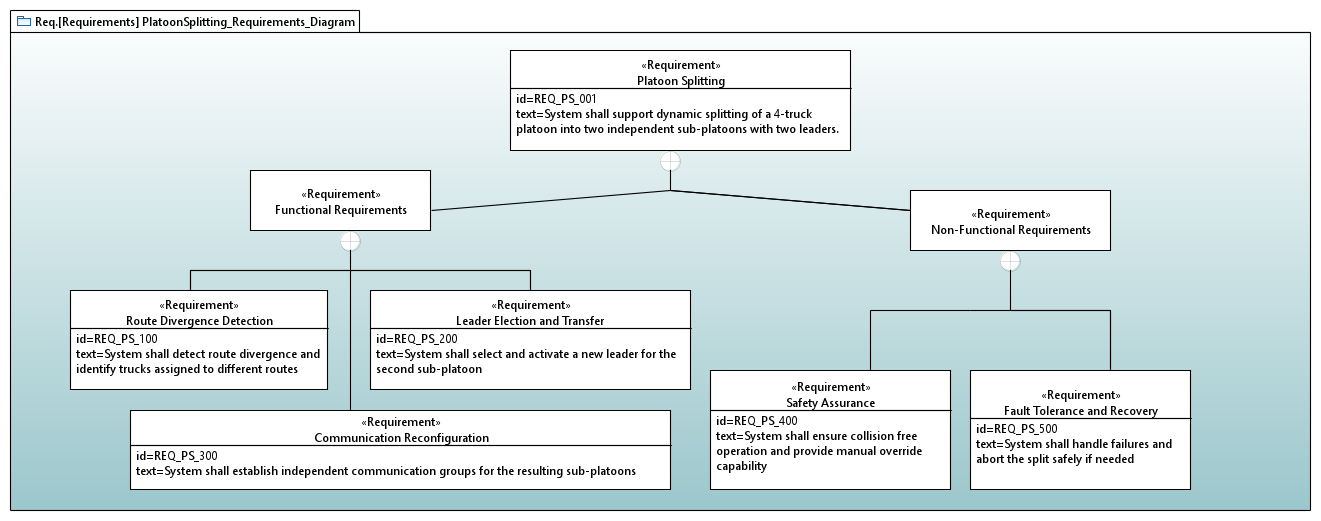
\includegraphics[width=0.65\textwidth]{figures/platoon_splitting_requirements.png}
\caption{SysML requirements diagram of the platoon splitting scenario.}
\label{fig:splitting-req}
\end{figure}

\begin{figure}[H]
\centering
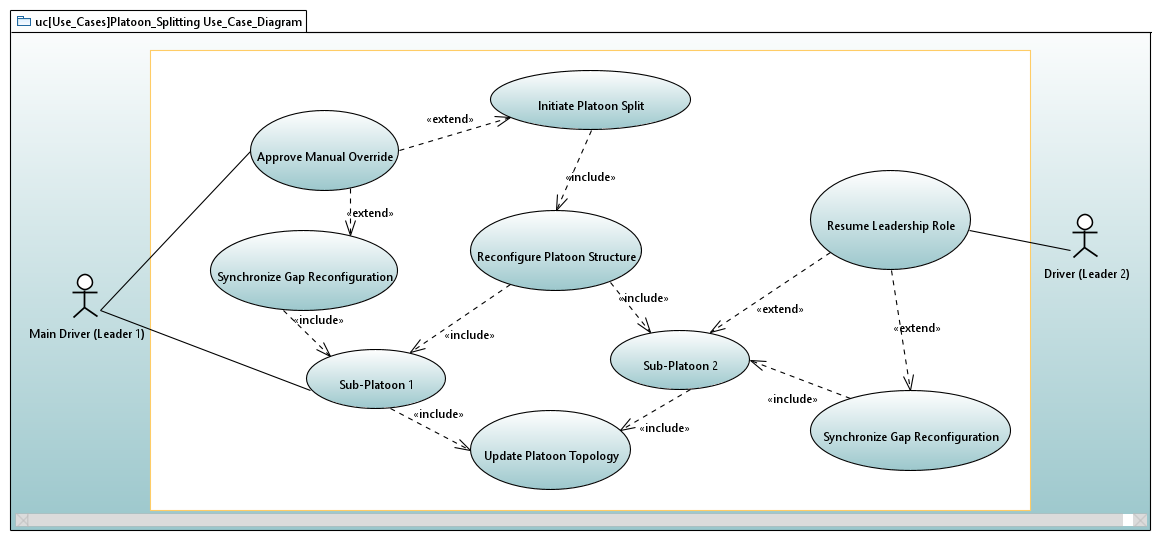
\includegraphics[width=0.65\textwidth]{figures/platoon_splitting_usecase.png}
\caption{SysML use case diagram of the platoon splitting scenario.}
\label{fig:splitting-usecase}
\end{figure}

\section{Communication Data, Signals, and Protocols}\label{sec:comm}
From the scenarios, the data exchanged between trucks (speed, position, lane, gap, status, capabilities), the required signals, and the triggering events were derived, and a protocol was specified per scenario. In the integrated model, communication is represented by nine synchronisation channels; Table~\ref{tab:channels} summarises the most important ones together with their timing constants.

\begin{table}[H]
\centering
\caption{Core channels of the integrated UPPAAL model.}
\label{tab:channels}
\begin{tabular}{llll}
\toprule
Channel & Sender $\rightarrow$ Receiver & Meaning & Timing \\
\midrule
\texttt{statusUpdate} & Lead $\rightarrow$ Follower & periodic status broadcast & $\leq 100$\,ms \\
\texttt{emergencyBrake} & Lead $\rightarrow$ all (broadcast) & emergency stop & $\leq 100$\,ms \\
\texttt{obstacleCleared} & Lead $\rightarrow$ all (broadcast) & resume operation & none \\
\texttt{gapTooSmall} & Distance ctrl.\ $\rightarrow$ Follower & unsafe gap detected & react $\leq 500$\,ms \\
\texttt{safeGapRestored} & Distance ctrl.\ $\rightarrow$ Follower & gap corrected & $\leq 500$\,ms \\
\texttt{commFailure} & Comm.\ monitor $\rightarrow$ Follower & V2V failure detected & timeout-based \\
\texttt{enterSafeMode} & Comm.\ monitor $\rightarrow$ Follower & activate fail-safe & guarded \\
\texttt{recoveryAttempt} & Comm.\ monitor $\rightarrow$ Follower & retry connection & every 10\,s \\
\texttt{commRestored} & Comm.\ monitor $\rightarrow$ Follower & link re-established & none \\
\bottomrule
\end{tabular}
\end{table}

Communication failure is treated as a normal part of the protocol design rather than as a rare exception: the emergency brake channel is declared as a \emph{broadcast} channel and can be received from every follower state, so a brake command is never blocked by an ongoing gap correction or recovery procedure.

\section{Control Behaviour and Formal Verification with UPPAAL}\label{sec:uppaal}

\subsection{Integrated Model}
UPPAAL is a widely used tool for the formal verification of real-time and cyber-physical systems, with recent applications including safety validation and failure diagnosis in autonomous vehicle systems \cite{GGK25}. The control behaviour of the platoon is captured in an integrated UPPAAL model of four parallel timed automata: \emph{LeadTruckControl} (periodic status broadcast, obstacle detection, emergency braking within \texttt{BRAKE\_TIME} $= 100$\,ms), \emph{FollowerTruckControl} (normal following, gap handling, emergency stop, safe mode, recovery), \emph{DistanceController} (detection and correction of unsafe gaps within \texttt{GAP\_TIME} $= 500$\,ms, tracked by a global \texttt{safeDistance} flag), and \emph{CommunicationMonitor} (failure detection, safe-mode activation, periodic recovery every \texttt{RECOVERY\_TIME} $= 10$\,s). Clock invariants bound the residence time in critical states, e.g.\ the safe mode is bounded by a total recovery budget, and safe-mode entry is guarded by \texttt{safeDistance} so that a truck never disengages normal control while the gap is unsafe. The lane keeping capability of the individual vehicle, provided by the SVR line follower of Section~\ref{sec:svm}, corresponds to the follower's \emph{NormalFollowing} behaviour.

\begin{figure}[H]
\centering
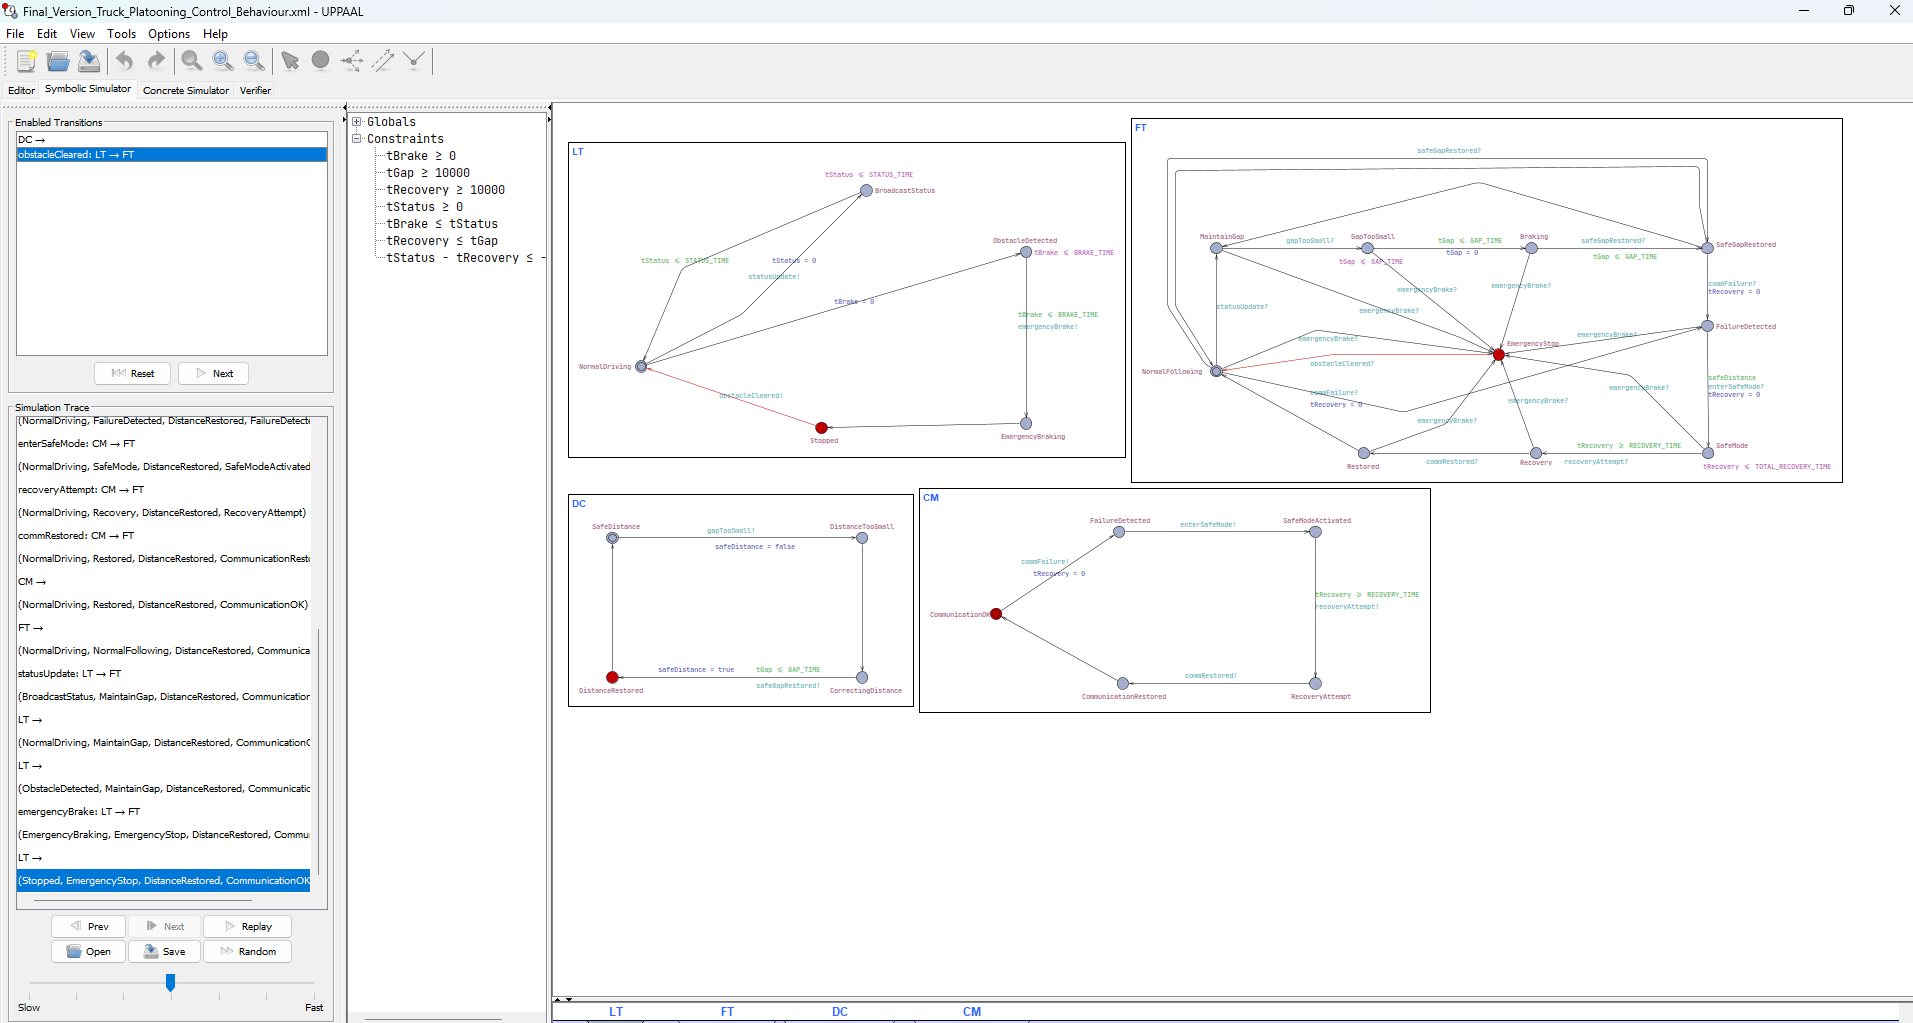
\includegraphics[width=0.95\textwidth]{figures/symbolic_simulator.png}
\caption{Symbolic simulation of the integrated platooning model in UPPAAL, showing all four automata (LeadTruckControl, FollowerTruckControl, DistanceController, CommunicationMonitor) and a simulation trace.}
\label{fig:symbolic}
\end{figure}

\needspace{8\baselineskip}
\subsection{Simulation and Verification Results}
The integrated model was exercised in the UPPAAL symbolic simulator (Figure~\ref{fig:symbolic}) for the nominal operation, gap-correction, communication-failure/recovery, and emergency-braking scenarios, including the critical combination of an emergency brake arriving while a follower is in safe mode or recovery. Two safety properties were checked with the UPPAAL model checker.

The central safety property,
\begin{center}
\texttt{A[] not deadlock},
\end{center}
was verified successfully (Figure~\ref{fig:verif-deadlock}): the platoon controller cannot reach a state in which no further progress is possible. Together with the state-based argument that \texttt{emergencyBrake} is receivable in every follower state, this establishes that the modelled platoon always remains reactive to emergency events.

\begin{figure}[H]
\centering
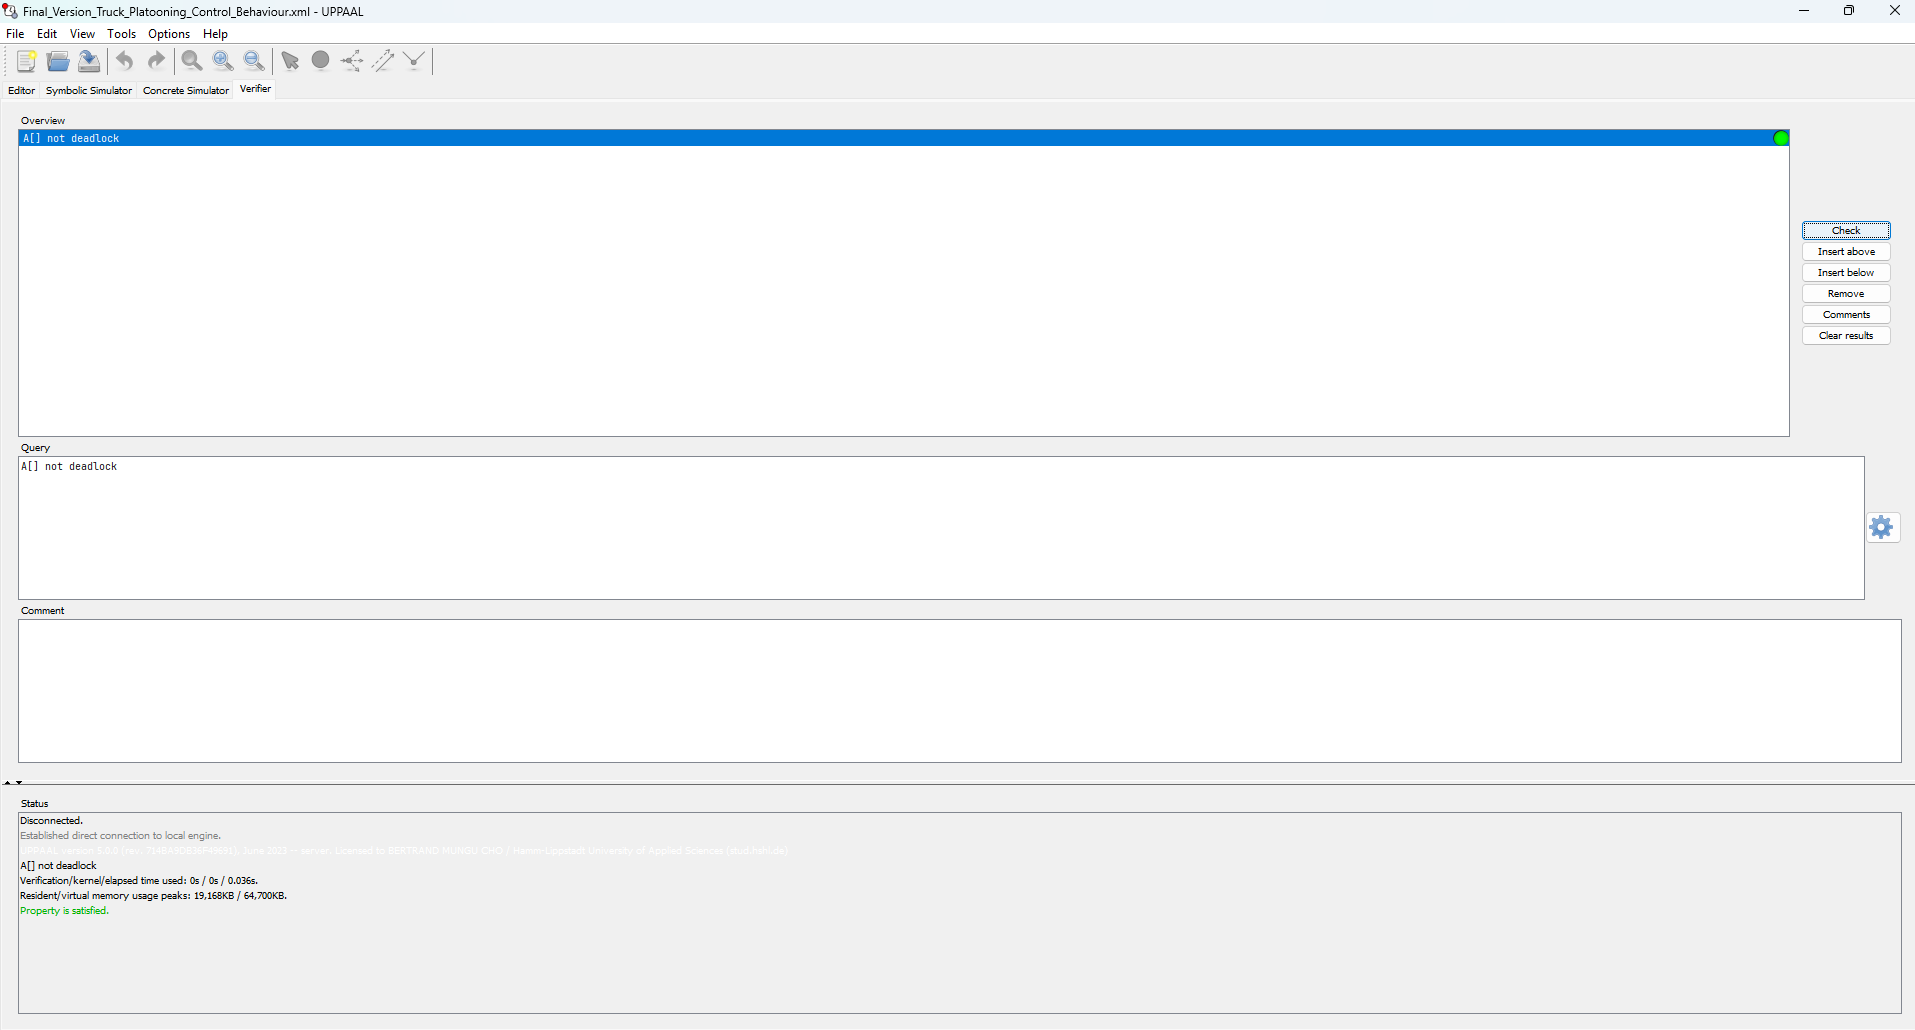
\includegraphics[width=0.95\textwidth]{figures/verifier_deadlock.png}
\caption{UPPAAL verifier result for \texttt{A[] not deadlock}: property satisfied.}
\label{fig:verif-deadlock}
\end{figure}

A second property checks the safe-mode guard discussed above: a follower must never be in safe mode while the distance controller reports an unsafe gap,
\begin{center}
\texttt{A[] !(FT.SafeMode \&\& DC.DistanceTooSmall)},
\end{center}
which was also verified successfully (Figure~\ref{fig:verif-safemode} in the appendix), confirming that the \texttt{safeDistance} guard on the transition into \texttt{SafeMode} works as intended across all reachable states of the integrated model.

\subsection{Challenges and Solutions}
The deadlock-free result above was not reached on the first attempt; earlier versions of the model had to be corrected in the following ways.

\textbf{Unreachable and deadlocking states.} Early follower automata modelled emergency braking as an ordinary transition available only from the normal-following state. This meant that a follower already reacting to a small gap or a communication failure could not receive the brake signal at all, and the model checker reported reachable deadlock states in exactly these combinations. The follower automaton was restructured so that \texttt{emergencyBrake} is a broadcast channel with a transition into \texttt{EmergencyStop} from every other state, removing the deadlock and matching the safety requirement that emergency braking must always take priority.

\textbf{Safe mode overriding an unsafe gap.} A related problem appeared when a communication failure and an unsafe following gap occurred together: the model allowed a truck to enter the low-priority safe mode while its gap to the truck ahead was still unsafe, effectively suppressing the more urgent gap-correction behaviour. This was fixed by guarding the transition into \texttt{SafeMode} with the global \texttt{safeDistance} flag, so a truck can only enter safe mode once it is confirmed to be at a safe distance.

\textbf{Scenario documentation drift.} While writing the four scenario descriptions in parallel, the communication-failure write-up initially drifted toward a differently themed intersection traffic-light example rather than the truck V2V communication case actually implemented in the UPPAAL model. This mismatch was caught during review and the scenario text was rewritten to describe the truck platooning communication failure that the \emph{CommunicationMonitor} automaton actually models, keeping the four scenario descriptions and the model consistent with each other.

\textbf{Shared channel names across scenarios.} Because each scenario was modelled independently by a different member, the channel names initially differed between the individual scenario files (Section~\ref{sec:comm}), which would have prevented them from being merged into one model. Before integration, the team agreed on one common set of channel names, listed in Table~\ref{tab:channels}, so the four independently developed automata could be combined into the single integrated model discussed above.

\needspace{10\baselineskip}
\section{Ask ChatGPT}
%% TODO: This section documents the mandatory AI-consultation exercise.
%% Replace the placeholder below with the actual question posed to ChatGPT and a
%% faithful summary or quotation of its answer, if the team used a different prompt.

\subsection{ChatGPT}
\textbf{Prompt to ChatGPT:} What role does formal verification play in the development of safety-critical cyber-physical systems such as autonomous vehicle platoons, and how does it complement machine learning components in the same system?

\textbf{ChatGPT said:} Formal verification plays a central role in safety-critical cyber-physical systems because it can mathematically prove that a system model satisfies given properties, such as the absence of deadlocks or the observance of timing bounds, across all possible execution paths rather than only the ones that were tested. This is especially important in domains like autonomous vehicle platooning, where a single missed edge case, such as an emergency brake signal arriving during an unrelated state transition, could have safety consequences. Machine learning components, such as perception or control models trained on data, are complementary but fundamentally different: they generalise well from examples but cannot offer the same exhaustive guarantees, since their behaviour on unseen inputs is not formally provable. A robust system architecture therefore typically separates concerns: learned components handle perception and control under normal operation, while a formally verified discrete controller enforces the hard safety envelope, such as emergency stopping or fallback behaviour, around them. This combination allows a system to benefit from the flexibility of learning while retaining checkable safety guarantees where they matter most.

\subsection{Scientific Discussion}
The answer correctly identifies the core distinction our project relies on: the SVR-based line follower (Section~\ref{sec:svm}) is a learned component that generalises from data and is evaluated statistically, whereas the UPPAAL model of the platoon control behaviour (Section~\ref{sec:uppaal}) is exhaustively checked against a formal property, \texttt{A[] not deadlock}, across the entire reachable state space rather than a finite set of test cases. This matches the architectural separation ChatGPT describes: the learned line follower governs the vehicle's \emph{NormalFollowing} behaviour, while the emergency braking, safe-mode, and distance-keeping logic that overrides it are captured as clock-constrained timed automata with explicit worst-case timing bounds (detection $\leq 50$\,ms, broadcast $\leq 100$\,ms, follower braking $\leq 150$\,ms, fallback $\leq 200$\,ms). However, the answer remains at a general, textbook level; it does not address concrete difficulties such as how to keep an evolving learned component and a fixed formal model consistent as the system is updated, or how to formally bound the behaviour of the learned component itself, which is an open research problem \cite{GGK25}. This illustrates that large language models are useful for orienting a design discussion and confirming that a chosen architecture follows established practice, but they do not replace the concrete engineering work of specifying timing constants, writing the automata, and running the model checker, which is where the actual safety guarantee in this project comes from.

\newpage
\section{Conclusion}
Across the two laboratories, the project covered the complete development process of an autonomous platooning system: the machine learning lab delivered a learned perception and control component validated on real hardware, and the cyber-physical systems lab built on it with scenario-based requirements engineering, SysML modelling, and a formally verified timed-automata model of the platoon coordination. The line follower achieved a test MAE of 0.0075 ($R^2 = 0.99$) under leakage-free temporal evaluation and performed among the top teams in the competition; the integrated UPPAAL model was proven deadlock-free while satisfying the specified timing structure.

\emph{Limitations.} The line follower was tuned and tested at moderate throttle; the PD gains for higher speed bands are conservative extrapolations and untested on the vehicle. The perception pipeline assumes a single green line and calibrated camera geometry. On the platooning side, the UPPAAL model abstracts from vehicle dynamics, message loss probabilities, and platoon size scaling ($N = 4$ trucks with a single modelled follower instance); the platoon formation and splitting protocols were modelled per scenario but not yet merged into the integrated verification model. Future work includes verifying additional safety and liveness queries, instantiating multiple follower processes, and integrating formation and splitting into the combined model.

\newpage
\section{Declaration of Originality}
We, Bertrand Mungu Cho, Daniel Chidi Chimezie, Riwaj Ghimire and Stephen Uzochi Obuh, herewith declare that we have composed the present paper and work by ourselves and without the use of any other than the cited sources and aids. Sentences or parts of sentences quoted literally are marked as such; other references with regard to the statement and scope are indicated by full details of the publications concerned. The paper and work in the same or similar form have not been submitted to any examination body and have not been published. This paper was not yet, even in part, used in another examination or as a course performance. We agree that our work may be checked by a plagiarism checker.

\paragraph{AI tools we have used:} Claude and ChatGPT were used to learn and understand concepts needed for this project, such as interpreting scikit-learn error messages, understanding \texttt{TimeSeriesSplit} behaviour, sanity-checking the geometric labeling formula, and troubleshooting the UPPAAL deadlock issues described in Section~6.3. ChatGPT was additionally consulted for the ``Ask ChatGPT'' exercise in Section~7.

\vspace*{3\baselineskip}

\noindent
\begin{minipage}[t]{0.48\textwidth}
\vspace*{4\baselineskip}
\hrule
\begin{tabular}{@{}p{1.8cm}p{3.4cm}@{}}
\small Date \& Place & \small\raggedleft\textit{Bertrand Mungu Cho}
\end{tabular}
\end{minipage}
\hfill
\begin{minipage}[t]{0.48\textwidth}
\vspace*{4\baselineskip}
\hrule
\begin{tabular}{@{}p{1.8cm}p{3.4cm}@{}}
\small Date \& Place & \small\raggedleft\textit{Daniel Chidi Chimezie}
\end{tabular}
\end{minipage}

\vspace*{3\baselineskip}

\noindent
\begin{minipage}[t]{0.48\textwidth}
\vspace*{4\baselineskip}
\hrule
\begin{tabular}{@{}p{1.8cm}p{3.4cm}@{}}
\small Date \& Place & \small\raggedleft\textit{Riwaj Ghimire}
\end{tabular}
\end{minipage}
\hfill
\begin{minipage}[t]{0.48\textwidth}
\vspace*{4\baselineskip}
\hrule
\begin{tabular}{@{}p{1.8cm}p{3.4cm}@{}}
\small Date \& Place & \small\raggedleft\textit{Stephen Uzochi Obuh}
\end{tabular}
\end{minipage}

\newpage
\bibliography{mybibfile}

\newpage
\appendix
\section{Appendix}\label{sec:appendix-all}

\subsection{Machine Learning Pipeline Figures}\label{sec:appendix}
This appendix collects supporting figures from the machine learning notebooks that back the numbers and claims made in Section~\ref{sec:svm}; the feature extraction pipeline (Figure~\ref{fig:mask-pipeline}) and the tuned model evaluation (Figure~\ref{fig:tuned-model}) are shown directly in that section.

\begin{figure}[H]
\centering
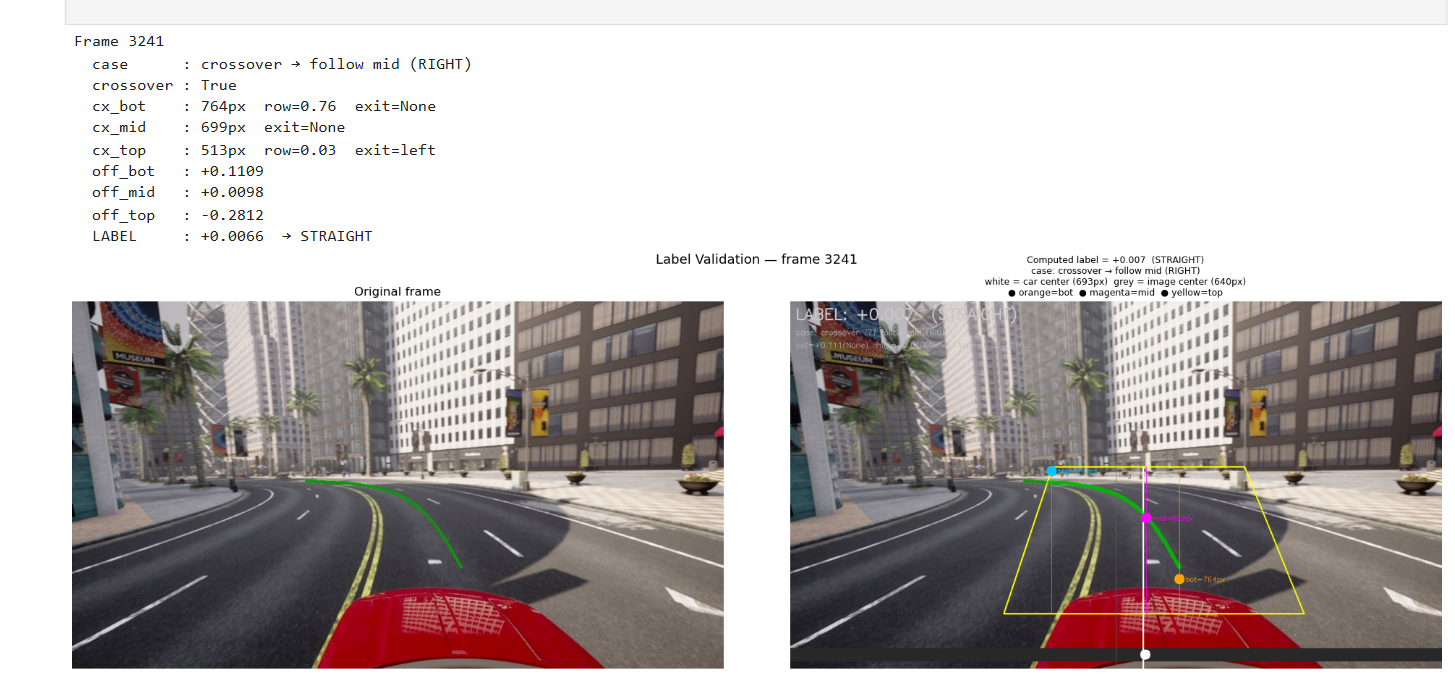
\includegraphics[width=0.9\textwidth]{figures/appendix_label_validation.png}
\caption{Geometric label computed for a single frame, overlaid on the original image for manual validation.}
\label{fig:app-label}
\end{figure}

\begin{figure}[H]
\centering
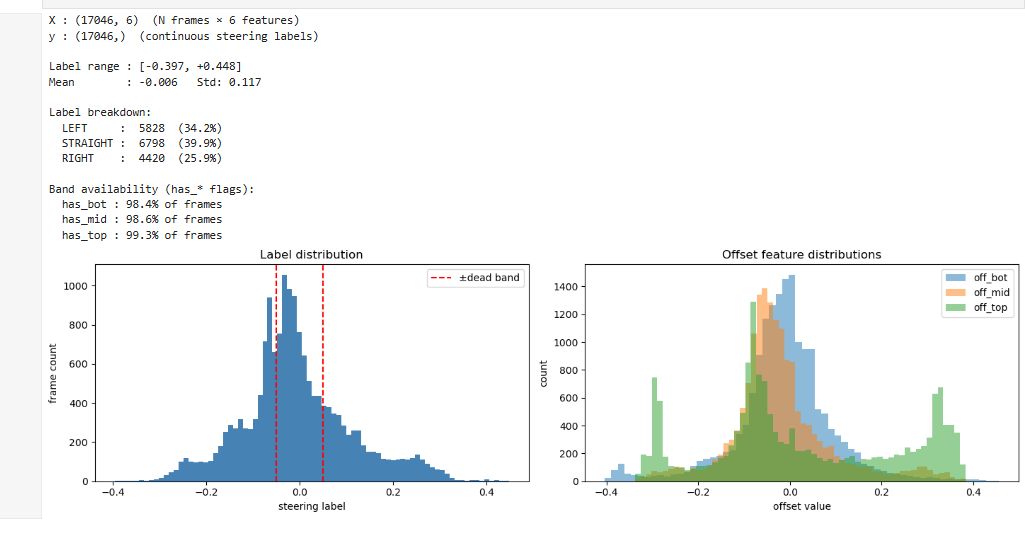
\includegraphics[width=0.85\textwidth]{figures/appendix_label_distribution.png}
\caption{Distribution of the continuous steering labels and of the three offset features across the dataset.}
\label{fig:app-dist}
\end{figure}

\begin{figure}[H]
\centering
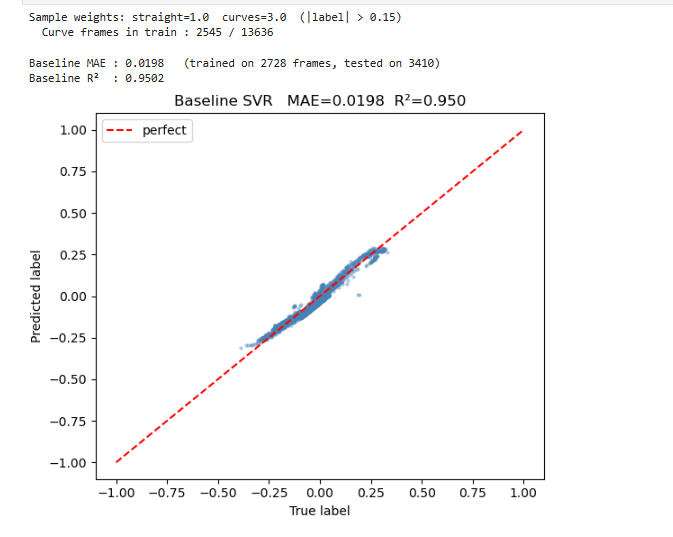
\includegraphics[width=0.75\textwidth]{figures/appendix_baseline_svr.png}
\caption{Predicted versus true steering label for the baseline SVR on the held-out test block.}
\label{fig:app-baseline}
\end{figure}

\begin{figure}[H]
\centering
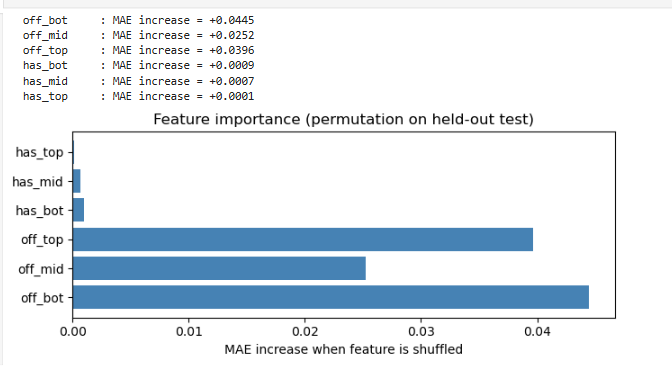
\includegraphics[width=0.75\textwidth]{figures/appendix_feature_importance.png}
\caption{Permutation feature importance of the tuned SVR on the held-out test block.}
\label{fig:app-importance}
\end{figure}

\subsection{Additional Truck Platooning Diagrams}\label{sec:appendix-platooning}
This appendix collects further SysML diagrams produced for the four platooning scenarios that are not shown in Section~\ref{sec:scenarios}, together with the diagram referenced there for platoon formation.

\begin{figure}[H]
\centering
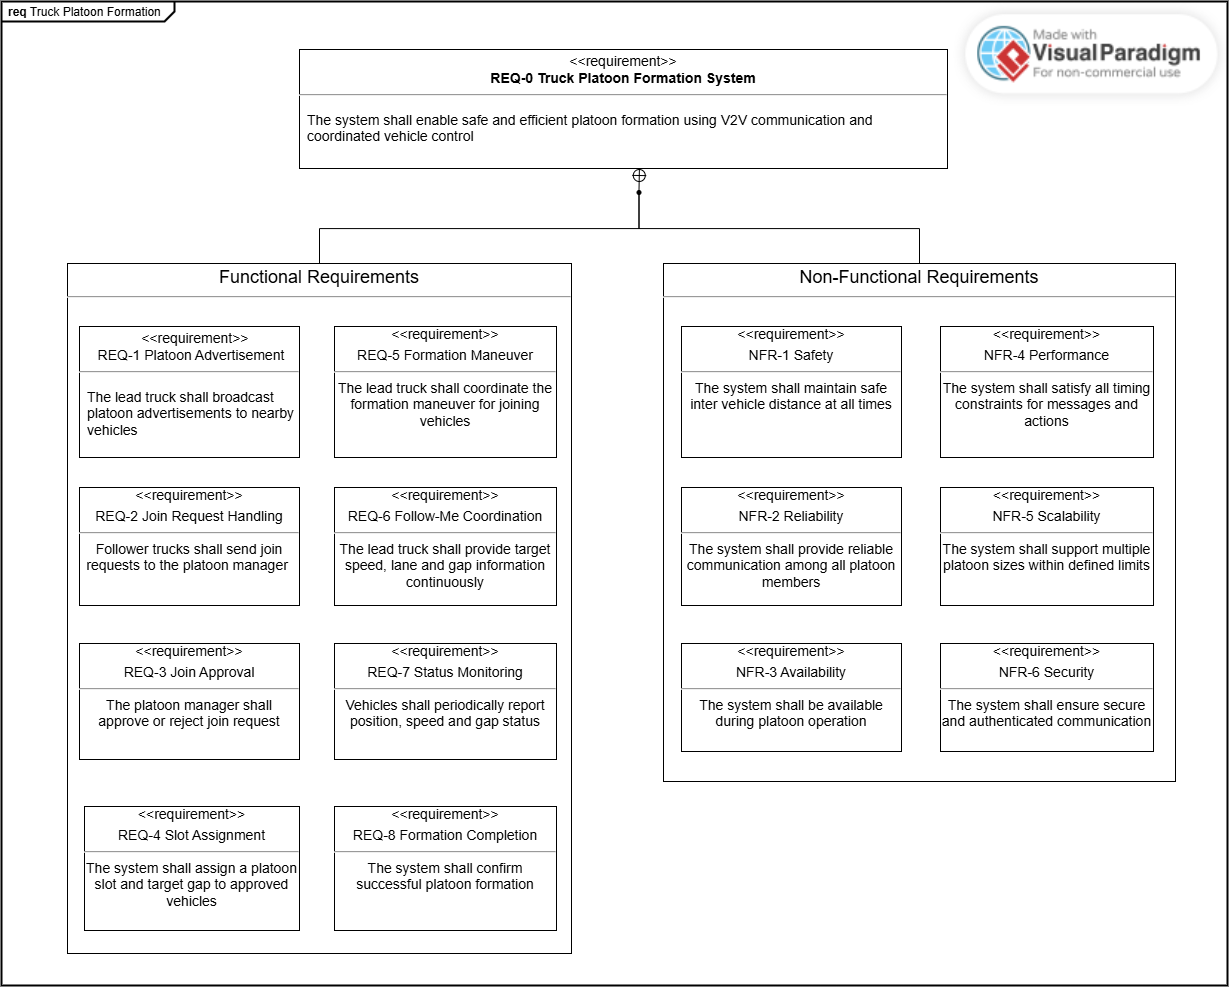
\includegraphics[width=0.5\textwidth]{figures/appendix_formation_requirements.png}
\caption{SysML requirement diagram of the platoon formation scenario.}
\label{fig:app-formation-req}
\end{figure}

\begin{figure}[H]
\centering
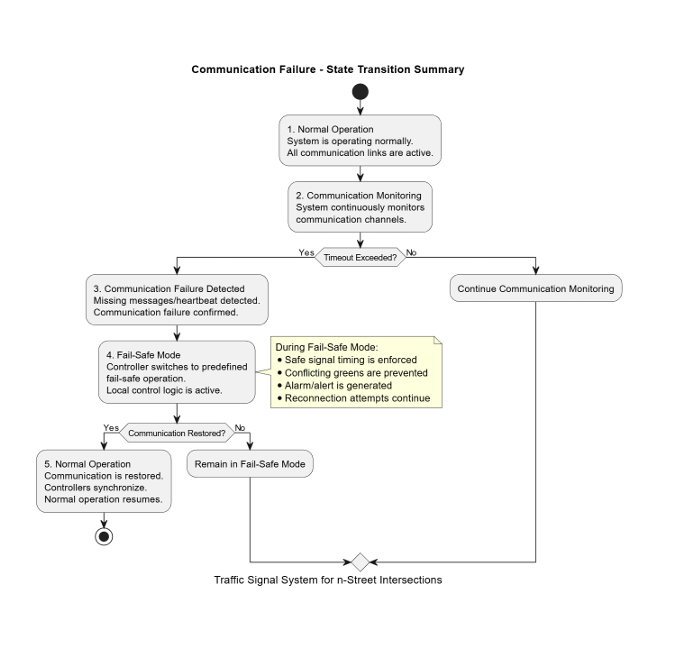
\includegraphics[width=0.62\textwidth]{figures/appendix_comm_failure_state_transition.png}
\caption{State transition diagram of the communication failure scenario.}
\label{fig:app-comm-failure-state}
\end{figure}

\begin{figure}[H]
\centering
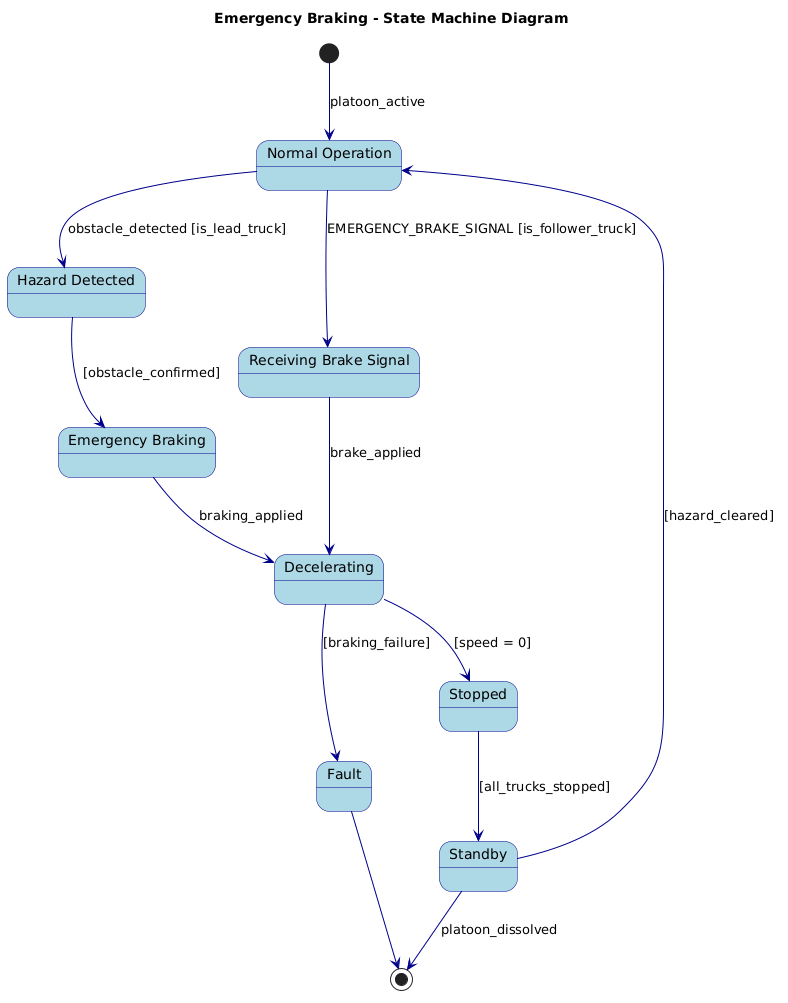
\includegraphics[width=0.55\textwidth]{figures/appendix_eb_state_machine.png}
\caption{State machine diagram of the emergency braking scenario.}
\label{fig:app-eb-state}
\end{figure}

\subsection{UPPAAL Model Details}\label{sec:appendix-uppaal}
This appendix collects additional details of the integrated UPPAAL model referenced in Section~\ref{sec:uppaal}.

\begin{figure}[H]
\centering
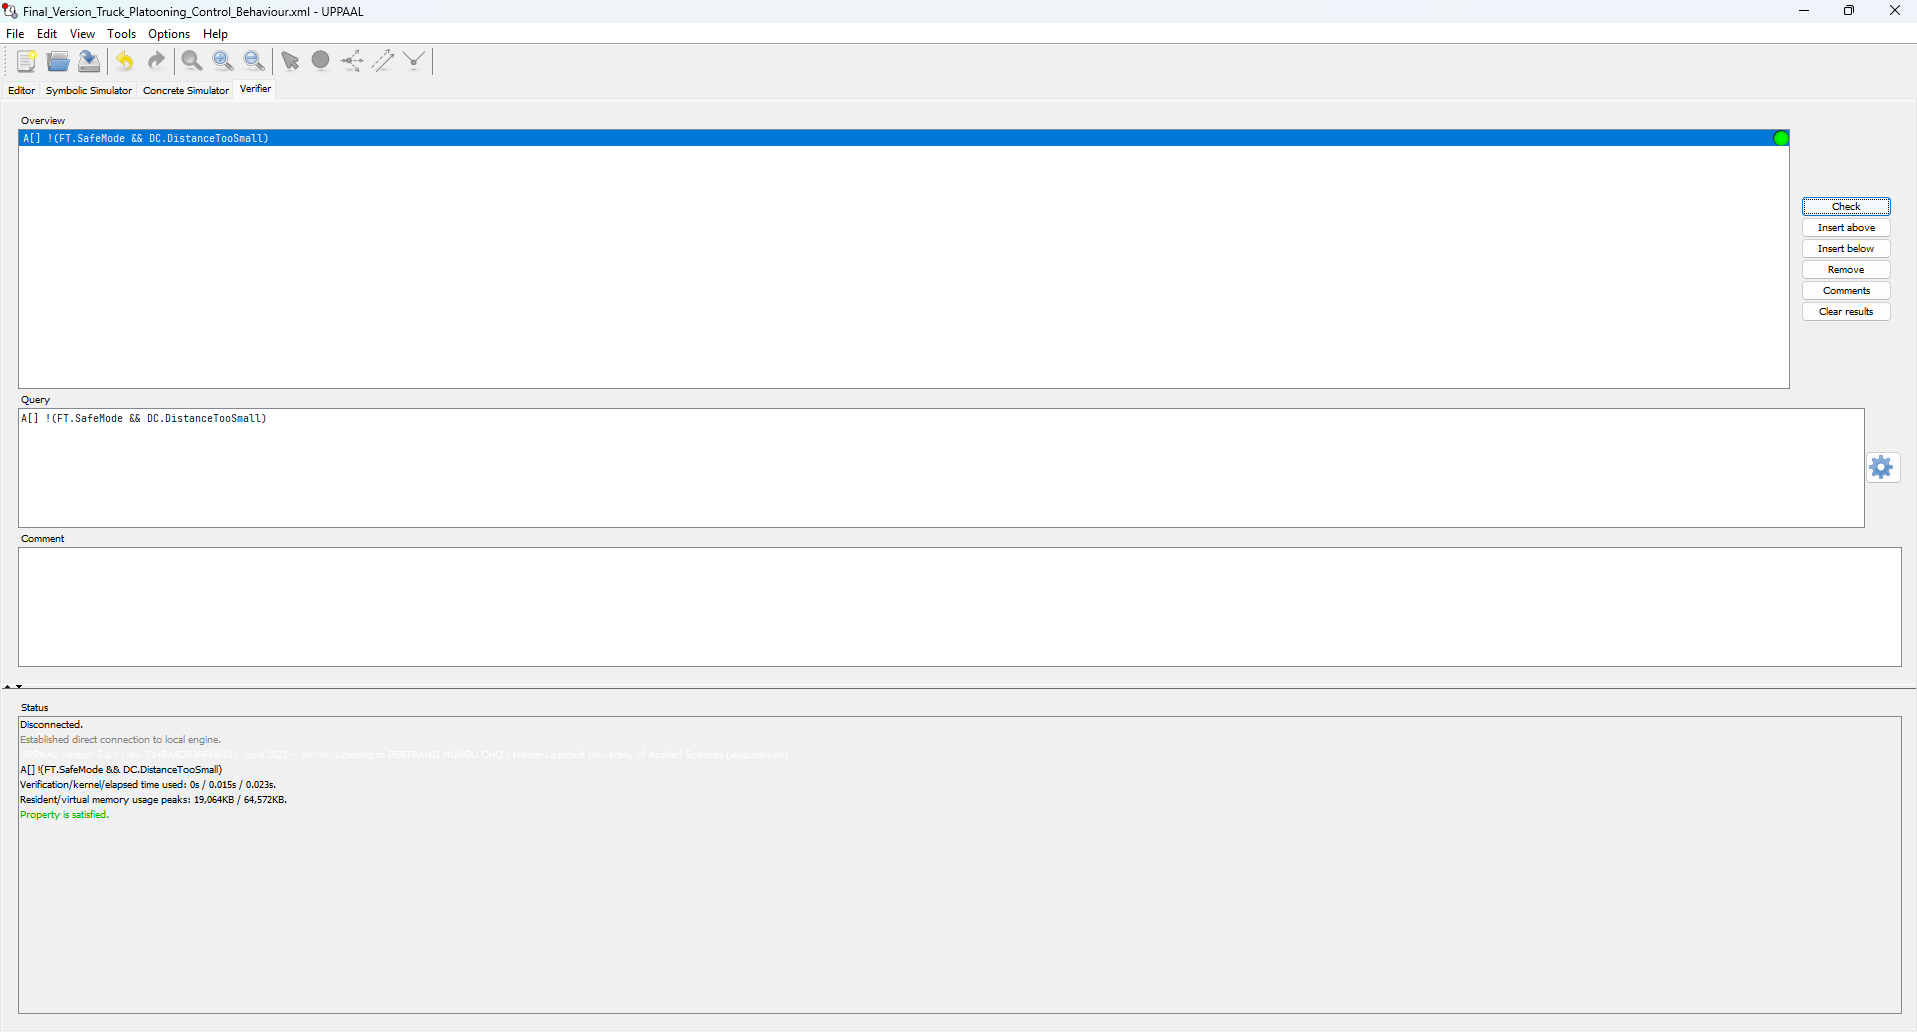
\includegraphics[width=0.7\textwidth]{figures/verifier_safemode_distance.png}
\caption{UPPAAL verifier result for \texttt{A[] !(FT.SafeMode \&\& DC.DistanceTooSmall)}: property satisfied.}
\label{fig:verif-safemode}
\end{figure}

The global declaration of the integrated model defines the synchronisation channels, constants, and clocks shared by all four automata (Listing~\ref{lst:global-decl}).

\begin{lstlisting}[caption={Global declaration of the integrated UPPAAL model.}, label={lst:global-decl}, basicstyle=\ttfamily\footnotesize, breaklines=true, frame=single, aboveskip=4pt, belowskip=4pt]
chan statusUpdate;
chan gapTooSmall;
chan safeGapRestored;
broadcast chan emergencyBrake;
chan commFailure;
chan enterSafeMode;
chan recoveryAttempt;
chan commRestored;
broadcast chan obstacleCleared;

const int N = 4;       // total trucks
const int F = N - 1;   // follower trucks

const int BRAKE_TIME = 100;
const int GAP_TIME = 500;
const int RECOVERY_TIME = 10000;
const int STATUS_TIME = 100;

const int TOTAL_GAP_TIME = GAP_TIME * N;
const int TOTAL_RECOVERY_TIME = RECOVERY_TIME * N;
bool safeDistance = true;

clock tBrake;
clock tGap;
clock tRecovery;
clock tStatus;
\end{lstlisting}

\end{document}
